\section{Hypothesis Testing}
\label{sect:hypothesis-testing}
\begin{enumerate}
\item Instead of \emph{estimating} the parameter \(\theta\), here we perform
some \emph{tests} on what the true parameter \(\theta\) could and could not
be.
\end{enumerate}
\subsection{Hypothesis Tests}
\begin{enumerate}
\item A \defn{hypothesis test} takes the following form:
\[
H_0: \theta\in\Theta_0\qqtext{vs.}H_1:\theta\in\Theta_1
\]
for some sets \(\Theta_0\) and \(\Theta_1\). Here, \(H_0\) is known as
\defn{null hypothesis} and \(H_1\) is known as \defn{alternative hypothesis}.

Each hypothesis postulates a range of possible values of true parameter
\(\theta\), and the main aim of hypothesis testing is to \emph{test} which
hypothesis (range) is \emph{more plausible}. \begin{warning}
``More plausible'' is \underline{not} the same as ``true''!
\end{warning}

\begin{note}
In general, the intersection \(\Theta_0\cap\Theta_1\) may be \emph{nonempty}
and the union \(\Theta_0\cup\Theta_1\) may \emph{not} be the whole parameter
space (i.e., set of all possible values of \(\theta\)). (But often both are the
cases.)
\end{note}
\item To conduct a hypothesis test, we seek for empirical data evidence from
the sample \(\vect{X}\) that supports {\color{red}\emph{rejection}} of null
hypothesis \(H_0\) {\color{ForestGreen}\emph{in favour of}} alternative
hypothesis \(H_1\). \begin{warning}
Again this does not mean alternative hypothesis \(H_1\) is \emph{true}!
\end{warning}

\begin{note}
When null hypothesis \(H_0\) is \emph{rejected} (i.e., values in \(\Theta_0\)
are deemed ``not plausible''), the values in \(\Theta_1\setminus\Theta_0\)
automatically become ``more plausible'' (due to having less ``competition'')
\faIcon{arrow-right} alternative hypothesis \(H_1\) becomes more
favourable/plausible (as long as \(\Theta_1\setminus\Theta_0\) is nonempty,
which is almost always the case).
\end{note}

\item When there is ``adequate'' evidence from \(\vect{X}\) that supports the
rejection, we \emph{reject} \(H_0\) in favour of \(H_1\) (or ``accept
\(H_1\)''). On the other hand, when there is ``inadequate'' evidence from
\(\vect{X}\) that supports the rejection, we \emph{do not reject} \(H_0\) (or
``accept \(H_0\)'').

\begin{warning}
Here, ``reject'' and ``accept'' do \underline{not} carry the meaning of
``declaring as false'' or ``declaring as true'' (respectively). Rather,
rejecting (accepting) a hypothesis here just means deeming the hypothesis as
``not plausible'' (``plausible'').
\end{warning}

\item More theoretically and mathematically, a hypothesis test can be described
as a \defn{test function} (or simply \defn{test}) \(\varphi\) defined
by
\[
\varphi(\vect{X})=\probtheta{\text{reject \(H_0\)}|\vect{X}}.
\]
\begin{note}
This means that we reject \(H_0\) with probability \(\varphi(\vect{X})\) when
the sample \(\vect{X}\) is observed (``unrealized'' case), or we reject \(H_0\)
with probability \(\varphi(\vect{x})\) when the sample \(\vect{X}=\vect{x}\) is
observed (``realized'' case).

More specifically, when the ``probability'' is one (zero), it simply means we
reject \(H_0\) (do not reject \(H_0\)) and the probabilistic meaning is gone.
\end{note}

\item A commonly seen form of test function (which is also our focus here) is given
by
\[
\varphi(\vect{X})=\indicset{\vect{X}\in\mathcal{C}}.
\]
where \(\indicset{\cdot}\) is the indicator function, and \(\mathcal{C}\) is
known as \defn{critical region} (or \defn{rejection region}).

\begin{remark}
\item This means we reject \(H_0\) iff \(\vect{X}\in\mathcal{C}\).
\item When \(\vect{X}=\vect{x}\) is observed, the test function is given by
\(\varphi(\vect{x})\), and so in this context \(H_0\) is rejected iff
\(\vect{x}\in\mathcal{C}\).
\end{remark}

\item When we reject \(H_0\), sometimes we call the evidence as
\defn{statistically significant}. Note that ``significant'' do \emph{not} carry
the meaning of ``importance'' here. Instead, it means the evidence
\emph{signifies} that \(H_0\) should be rejected (it is adequate for supporting
the rejection).

\begin{note}
Likewise, when an evidence is called \defn{statistically insignificant}, it
just means that the evidence does \emph{not} signify that \(H_0\) should be
rejected.
\end{note}

\item A common form of the critical region \(\mathcal{C}\) is
\[
\mathcal{C}=\{\vect{X}:T(\vect{X})>c\}\quad(\text{or simply \(\{T(\vect{X})>c\}\)})
\]
where \(T=T(\vect{X})\) is a statistic (known as \defn{test statistic}) and
\(c\) is a constant (known as \defn{critical value}). In this case, we reject
\(H_0\) iff \(T(\vect{X})>c\).

\begin{remark}
\item The inequality ``\(>\)'' can be replaced by ``\(<\)'', ``\(\le\)'', or ``\(\ge\)''.
\item When \(\vect{X}=\vect{x}\) is observed, the critical region would be
modified to \(\{\vect{x}:T(\vect{x})>c\}\) (similar for critical regions with
other kinds of inequalities).
\end{remark}
\end{enumerate}

\subsection{Quality of a Hypothesis Test}
\begin{enumerate}
\item To assess the quality/``goodness'' of a test \(\varphi\), we mainly use
two metrics: \emph{size} and \emph{power}. Before discussing them, let us first
introduce a preliminary concept: \emph{power function} (not to be confused with
\emph{power}!).

\item The \defn{power function} of a test \(\varphi\) is
\[
w_{\varphi}(\theta)=\expvtheta{\varphi(\vect{X})}
=\expvtheta{\probtheta{\text{reject \(H_0\)}|\vect{X}}}
=\probtheta{\text{reject \(H_0\)}}
\]
where the last equality follows from law of total expectation.

\item When \(\theta\in\Theta_0\) (\(H_0\) is true), the power function is
\(w_{\varphi}(\theta)=\probtheta{\text{reject true \(H_0\)}}\), and when
\(\theta\in\Theta_1\setminus\Theta_0\) (assuming \(\Theta_1\setminus\Theta_0\)
is nonempty), the power function is \(w_{\varphi}(\theta)=1-\probtheta{\text{not
reject false \(H_0\)}}\).

The act of rejecting true \(H_0\) is known as \defn{type I error}, and the act
of not rejecting false \(H_0\) is known as \defn{type II error}.

\item The \defn{size} of a test \(\varphi\) is
\(\sup\{w_{\varphi}(\theta):\theta\in\Theta_0\}\) (or
\(\displaystyle \sup_{\theta\in\Theta_0}\{w_{\varphi}(\theta)\}\)), which can be loosely
interpreted as the ``worse'' (``highest'') type I error probability. This is
also known as the \defn{significance level} of the test \(\varphi\).

\item The \defn{power} of a test \(\varphi\) at
\(\theta\in\Theta_1\setminus\Theta_0\) is given by the output of power function
at \(\theta\): \(w_{\varphi}(\theta)\). This can be interpreted as \(1-\text{type II
error probability}\).

\item The \emph{smaller} the size and the \emph{larger} the power at each
\(\theta\in\Theta_1\setminus\Theta_0\) (i.e., type I and II errors are both
smaller), the \emph{better} the test. Then, it may seem that the ``optimal''
test is the one that simultaneously achieves the smallest size and the largest
power at each \(\theta\in\Theta_1\setminus\Theta_0\).

\item \label{it:size-power-inverse-relate}
Unfortunately, we cannot get ``the best of both worlds'' in general since often
reducing the size would lead to reduction in power also (and increasing the
power would lead to increase in size also).

\begin{intuition}
When we try to reduce the size, the test becomes more ``conservative''
(requiring \emph{very strong} evidence for rejecting \(H_0\))
\faIcon{arrow-right} avoiding much type I error, but also raising type
II error.

On the other hand, when we try to increase the power, the test becomes more
``aggressive'' (requiring rather weak evidence for rejecting \(H_0\))
\faIcon{arrow-right} rejecting \(H_0\) frequently \faIcon{arrow-right} avoiding
much type II error, but also raising type I error.
\end{intuition}

\item \label{it:good-test-goal}
Due to the constraint in \labelcref{it:size-power-inverse-relate}, we
usually seek a test \(\varphi\) whose size is (at most) a certain predetermined
level \(\alpha\) and whose power is \emph{as large as possible} for every
\(\theta\in\Theta_1\setminus\Theta_0\) \faIcon{arrow-right} type I error
probability has been controlled, and we try to reduce type II error as far as
possible (or in other words, increase the power as far as possible).

\begin{note}
Note that when we consider \emph{power} of a test, we focus on
\(\Theta_1\setminus\Theta_0\) rather than \(\Theta_1\) (just the parameter
values appearing \emph{exclusively} in \(H_1\)). Consequently, even if one
modifies the alternative hypothesis to
\(H_1:\theta\in\Theta_1\setminus\Theta_0\), there is not much ``material''
effect, and often the previous results would still hold. Thus, we usually treat
the tests before and after this modification as interchangeable.
\end{note}
\end{enumerate}
\subsection{\(p\)-value}
\begin{enumerate}
\item A frequently seen jargon in statistical inference is \emph{\(p\)-value}
(which is unfortunately a confusing concept to many people!).

\item In the  discussion of \(p\)-value here, we shall focus on the typical
case where the test function is
\(\varphi(\vect{X})=\indicset{\vect{X}\in\mathcal{C}}\).

\item When \(\vect{X}=\vect{x}\) is observed, the \defn{\(p\)-value}, denoted
by \(\operatorname{pv}(\vect{x})\), is the ``\emph{smallest}'' possible size for a test
\(\varphi\) while retaining \(\varphi(\vect{x})=1\) (i.e., the test suggests
rejection of \(H_0\)).

\begin{note}
The term ``smallest'' is not very accurate technically. More precisely, the
\(p\)-value \(\operatorname{pv}(\vect{x})\) is the \emph{infimum}
\[
\inf\{\text{size of \(\varphi\)}:\text{\(\varphi\) is a test with \(\varphi(\vect{x})=1\)}\}.
\]
\end{note}

\begin{intuition}
When \(\vect{X}=\vect{x}\) is observed, the \(p\)-value
\(\operatorname{pv}(\vect{x})\) indicates the size of the ``most conservative
test''\footnote{Here, ``more conservative'' \faIcon{arrows-alt-h} more
``prudent'' in rejecting \(H_0\) (requiring ``stronger'' evidence)
\faIcon{arrows-alt-h} smaller size. So, ``most conservative''
\faIcon{arrows-alt-h} ``smallest size''.} we can use to reject \(H_0\) based on
\(\vect{x}\).

Now, if the \(p\)-value \(\operatorname{pv}(\vect{x})\) is very small, it
suggests that the size of the ``most conservative test'' is very small
\faIcon{arrow-right} the ``most conservative test'' we can use to reject
\(H_0\) based on \(\vect{x}\) is really ``very conservative''
\faIcon{arrow-right} evidence contained in \(\vect{x}\) is really strong (even
``very conservative'' test rejects \(H_0\)).

Hence, the \(p\)-value \(\operatorname{pv}(\vect{x})\) also measures the
``strength'' of evidence contained in \(\vect{x}\) (smaller
\(\operatorname{pv}(\vect{x})\) \faIcon{arrow-right} stronger evidence
contained).
\end{intuition}

\item The main usage of \(p\)-value is to provide an alternative way to decide
whether \(H_0\) is rejected (as an alternative to checking whether
\(\varphi(\vect{x})=1\), i.e., whether \(\vect{x}\in\mathcal{C}\)), when
\(\vect{X}=\vect{x}\) is observed. The alternative method is as follows.
\begin{proposition}
\label{prp:p-val-decision}
Suppose that \(\vect{X}=\vect{x}\) is observed.  Focus on any collection of tests
in which a test with higher size does not have smaller \(\varphi(\vect{x})\).
Then, the null hypothesis \(H_0\) is rejected at significance level
\(\alpha\)\footnote{That is, the test is of significance level/size
\(\alpha\).} iff the \(p\)-value \(\operatorname{pv}(\vect{x})\le\alpha\).
\end{proposition}
\begin{pf}
\begin{center}
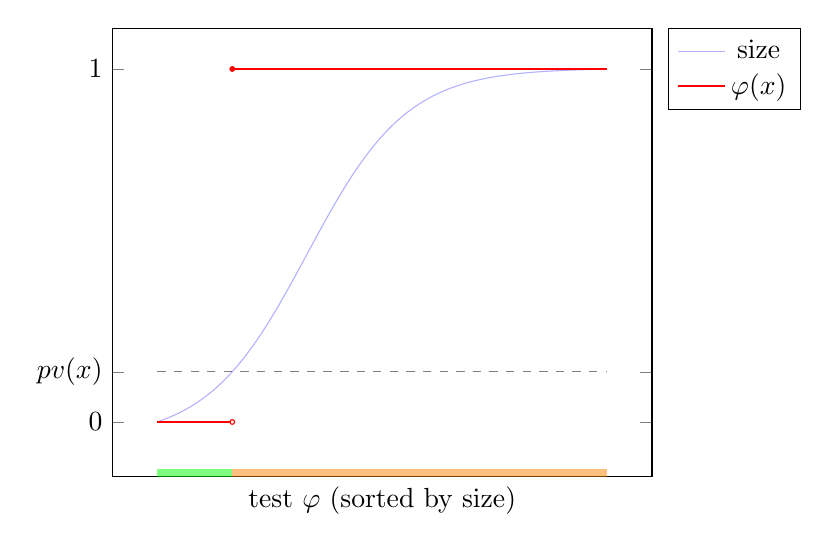
\begin{tikzpicture}
\begin{axis}[domain=0:3, samples=100, xtick=\empty, ytick={0.047,0.182, 0.998},
yticklabels={0,\(\operatorname{pv}(\vect{x})\),1},
xlabel={test \(\varphi\) (sorted by size)},
legend entries={size, \(\varphi(\vect{x})\)}, legend style={legend pos=outer north east},
ymin=-0.1
]
\addplot[blue, opacity=0.3]{1/(1+e^(-3*(x-1)))};
\addplot[red, domain=0:0.49]{0.047};
\addplot[red, domain=0.5:3]{0.998};
\addplot[black, dashed, opacity=0.5]{0.182};
\draw[red] (0.5,0.047) circle [radius=0.3mm];
\draw[red, fill] (0.5,0.998) circle [radius=0.3mm];
\draw[opacity=0.5, orange, line width=0.2cm] (0.5,-0.1) -- (3,-0.1);
\draw[opacity=0.5, green, line width=0.2cm] (0,-0.1) -- (0.5,-0.1);
\end{axis}
\end{tikzpicture}
\end{center}
The key observation is that for such collection of tests, the {\color{red}red}
function \(\varphi\mapsto\varphi(\vect{x})\) above is ``nondecreasing'' (as test
\(\varphi\) with higher size does not have smaller \(\varphi(\vect{x})\)).

Consequently, for any test with size
\(\alpha\ge\operatorname{pv}(\vect{x})\) ({\color{orange}orange} highlighted),
\(H_0\) is rejected, and for any test with size
\(\alpha<\operatorname{pv}(\vect{x})\) ({\color{green}green} highlighted),
\(H_0\) is not rejected.

\end{pf}

\begin{note}
In most cases of practical interest, the collection of tests focused
satisfies the condition imposed here, and thus this alternative method can be
utilized.  Indeed, this often serves as the main/standard approach for deciding
whether \(H_0\) is rejected when a computer can be used to calculate
\(p\)-values.
\end{note}
\item \label{it:p-val-fmlas}
The following give some commonly seen/conventional formulas related to
\(p\)-value:
\begin{enumerate}
\item Focusing on tests having critical region of the form \(\{T(\vect{X})>c\}\):
\[
\operatorname{pv}(\vect{x})=\inf_{c<T(\vect{x})}\sup_{\theta\in\Theta_0}
\underbrace{\expvtheta{\varphi(\vect{X})}}_{\probtheta{T(\vect{X})>c}}
=\sup_{\theta\in\Theta_0}\underbrace{\inf_{c<T(\vect{x})}\probtheta{T(\vect{X})>c}}_{\probtheta{T(\vect{X})\ge T(\vect{x})}}
=\boxed{\sup_{\theta\in\Theta_0}\probtheta{T(\vect{X})\ge T(\vect{x})}}.
\]

\item Focusing on tests having critical region of the form \(\{T(\vect{X})<c\}\):
\[
\operatorname{pv}(\vect{x})=\inf_{c>T(\vect{x})}\sup_{\theta\in\Theta_0}
\underbrace{\expvtheta{\varphi(\vect{X})}}_{\probtheta{T(\vect{X})<c}}
=\sup_{\theta\in\Theta_0}\underbrace{\inf_{c>T(\vect{x})}\probtheta{T(\vect{X})<c}}_{\probtheta{T(\vect{X})\le T(\vect{x})}}
=\boxed{\sup_{\theta\in\Theta_0}\probtheta{T(\vect{X})\le T(\vect{x})}}.
\]

\item Focusing on tests having critical region of the form \(\{|T(\vect{X})| >c\}\):
\[
\operatorname{pv}(\vect{x})=\inf_{c<|T(\vect{x})|}\sup_{\theta\in\Theta_0}
\underbrace{\expvtheta{\varphi(\vect{X})}}_{\probtheta{|T(\vect{X})|>c}}
=\sup_{\theta\in\Theta_0}\underbrace{\inf_{c<|T(\vect{x})|}\probtheta{|T(\vect{X})|>c}}_{\probtheta{|T(\vect{X})|\ge |T(\vect{x})|}}
=\boxed{\sup_{\theta\in\Theta_0}\probtheta{|T(\vect{X})|\ge |T(\vect{x})|}}.
\]
\end{enumerate}
\begin{mnemonic}
Replacing the ``\(c\)'' in the expression for critical region by
\(T(\vect{x})\) (or \(|T(\vect{x})|\)) gives the expression inside
\(\probtheta{\cdot}\) in each of the formula.
\end{mnemonic}

\begin{remark}
\item Recall that \(\displaystyle
\sup_{\theta\in\Theta_0}\expvtheta{\varphi(\vect{X})}\) is the size of the test
\(\varphi\).
\item Here we assume that ``\(\sup\)'' and ``\(\inf\)'' can be swapped without
affecting the value (this holds under some nice cases, and this case is one of
them).
\item The same formulas still hold when we replace ``\(>\)'' (``\(<\)'') by
``\(\ge\)'' (``\(\le\)'') in the critical regions.
\item In general, even with these formulas, it is quite hard to compute
\(p\)-values by hand. (But they are helpful for obtaining \(p\)-values by
computer.)
\end{remark}

\end{enumerate}

\subsection{Uniformly Most Powerful Test}
\begin{enumerate}
\item Based on the idea in \labelcref{it:good-test-goal}, we can characterize
an \emph{optimal} test in the sense of the notion in \labelcref{it:good-test-goal}.
Such test is known as \emph{uniformly most powerful test}.

\item A test \(\varphi_0\) is \defn{uniformly most powerful} (UMP) of size
\(\alpha\) if
\begin{itemize}
\item \(\varphi_0\) is of size \(\alpha\);
\item the power function \(w_{\varphi_0}(\theta)\ge w_{\varphi}(\theta)\) for
any \(\theta\in\Theta_1\setminus\Theta_0\) and any test \(\varphi\) of size \(\le\alpha\).
\end{itemize}
\begin{remark}
\item UMP test may not exist. But if it exists, then it is a desirable test.
\item The word ``uniformly'' reflects that the inequality holds for
\emph{every} \(\theta\in\Theta_1\setminus\Theta_0\) (not just a particular
\(\theta\)). In case \(\Theta_0=\{\theta_0\}\) and \(\Theta_1=\{\theta_1\}\)
(with \(\theta_0\neq\theta_1\)), we can drop the word ``uniformly'' and just
call the test \(\varphi_0\) \defn{most powerful} (MP) of size \(\alpha\).
\end{remark}
\end{enumerate}

\subsection{Likelihood Ratio Test}
\begin{enumerate}
\item An important kind of hypothesis test which possesses some nice properties
is \emph{likelihood ratio test}. As its name suggests, it involves a ``ratio
of likelihood functions'' (as test statistic).

\item For a hypothesis test with
\(H_0:\theta\in\Theta_0\qqtext{vs.}H_1:\theta\in\Theta_1\), the
\defn{likelihood ratio} for this test given sample \(\vect{X}\) is
\[
\Lambda_{\vect{X}}(H_0,H_1)=\frac{\displaystyle \sup_{\theta\in\Theta_1}\lik{\vect{X}}{\theta}}
{\displaystyle \sup_{\theta\in\Theta_0}\lik{\vect{X}}{\theta}}
\]
where \(\lik{\vect{X}}{\theta}\) is the likelihood function of \(\theta\) given
\(\vect{X}\).

\begin{remark}
\item The likelihood ratio measures the ``strength of evidence'' provided by
\(\vect{X}\) against \(H_0\) in favour of \(H_1\). (Higher value
\faIcon{arrow-right} ``stronger'' evidence.)
\item Roughly, the likelihood ratio means the ``odds'' of \(H_1\) against
\(H_0\): When it is higher, there is a higher ``tendency'' to reject \(H_0\) in
favour of \(H_1\).
\end{remark}
\item After having the likelihood ratio, we can use it as test statistic to
obtain a \defn{likelihood ratio test} which is a test with critical region
\[
\mathcal{C}=\{\vect{X}:\Lambda_{\vect{X}}(H_0,H_1)>c\}
\]
where \(c>0\) is a constant.

\item As a special case, when \(\Theta_0=\{\theta_0\}\) and
\(\Theta_1=\{\theta_1\}\), the critical region for likelihood ratio test takes
the form
\[
\mathcal{C}=\qty{\vect{X}:\frac{\lik{\vect{X}}{\theta_1}}{\lik{\vect{X}}{\theta_0}}>c}
\]
where \(c>0\) is a constant.
In this case, the likelihood ratio test is proven to be UMP by the following
result.
\begin{theorem}[Neyman-Pearson lemma]
\label{thm:neyman-pearson}
The likelihood ratio test in this special case, with size \(\alpha\), is UMP of
size \(\alpha\).
\end{theorem}
\end{enumerate}
\subsection{Tests Based on Asymptotic Theory}
\begin{enumerate}
\item Suppose that there are infinitely many independent \emph{but not
necessarily identically distributed} random variables \(X_1,X_2,\dotsc\) to be
included in a ``sample'' (technically due to the lack of identically
distributed property, it is not really a sample).

Now, for any \(n\in\N\), consider the ``sample'' \((X_1,\dotsc,X_n)\), and
suppose that its joint probability function can be expressed as a product of
marginal probability functions as follows:
\[
p_1(x_1|\theta)\times\dotsb\times p_n(x_n|\theta),
\]
where \(\theta\in\Theta\subseteq\R^r\) is a \emph{vector}.
\item Then, consider the hypothesis test
\[
H_0:\theta\in\Theta_0\qqtext{vs.}H_1:\theta\in\Theta_1
\]
where \(\Theta_0\subseteq\Theta_1\subseteq\R^r\), and \(\Theta_0\) and \(\Theta_1\)
have \(s\) and \(r\) \emph{degrees of freedom} with \(s<r\).

\begin{note}
Informally, degree of freedoms is the number of ``free'' parameters available.
For example, since \(\Theta_0\) has \(s\) degrees of freedom, although every
vector in \(\Theta_0\) has \(r>s\) entries, 
\end{note}

\item Let \(\widehat{\theta}_n\) and \(\widetilde{\theta}_n\) be the MLE of
\(\theta\) under \(H_1\) (over \(\Theta_1\supseteq\Theta_0\)) and the \emph{constrained} MLE of
\(\theta\) under \(H_0\) (only the values in \(\Theta_0\) are admissible)
respectively. Then, the \defn{generalized likelihood ratio} for this test given
sample \(\vect{X}\) is
\[
2\ln\Lambda_{\vect{X}}(H_0, H_1)=
2\ln\qty[\frac{\displaystyle \sup_{\theta\in\Theta_1}\lik{\vect{X}}{\theta}}
{\displaystyle \sup_{\theta\in\Theta_0}\lik{\vect{X}}{\theta}}]
=2\ln\qty[\frac{\lik{\vect{X}}{\widehat{\theta}_n}}{\lik{\vect{X}}{\widetilde{\theta}_n}}]
=2\qty[\sum_{i=1}^{n}\ln p_i\qty(X_i|\widehat{\theta}_n)
+\sum_{i=1}^{n}\ln p_i\qty(X_i|\widetilde{\theta}_n)]
\]
where \(\Lambda_{\vect{X}}(H_0, H_1)\) is the likelihood ratio for the test
given sample \(\vect{X}\).

\item The following result provides a basis for using the generalized
likelihood ratio as ``asymptotic'' test statistic.

\begin{theorem}[Wilks' theorem]
\label{thm:wilks}
Under \emph{regularity conditions}\footnote{We shall omit the technical details
here.} and if the null hypothesis \(H_0\) is true (i.e, \(\theta\in\Theta_0\)),
\[
\{2\ln\Lambda_{\vect{X}}(H_0, H_1)\}\convd\chi^2_{r-s}.
\]
\begin{note}
Recall that \(r\) and \(s\) are degrees of freedom for \(\Theta_1\) and
\(\Theta_0\) respectively.
\end{note}
\end{theorem}

\item Now, based on Wilks' theorem, we can construct a \defn{generalized
likelihood ratio test} which has the critical region
\[
\mathcal{C}=\{\vect{X}:2\ln\Lambda_{\vect{X}}(H_0, H_1)>\chi^2_{r-s}(\alpha)\}
\]
where \(\chi^2_{r-s}(\alpha)\) is the \(\alpha\)th upper quantile of the
distribution \(\chi^2_{r-s}\). This test is \emph{approximately} size
\(\alpha\) if \(n\) is large (we shall assume that the regularity conditions are
satisfied).


\item Consider a special case where \(\Theta_0=\{\theta_0\}\). Then, we can
write the hypothesis test as
\[
H_0:\theta=\theta_0\qqtext{vs.}H_1:\theta\in\Theta.
\]
\begin{note}
More commonly, we consider instead the hypothesis test
\[
H_0:\theta=\theta_0\qqtext{vs.}H_1:\theta\ne\theta_0
\]
where the alternative hypothesis is modified to \(H_1:
\theta\in\Theta_1\setminus\{\theta_0\}\). As mentioned previously, these two
tests can be regarded as interchangeable, so the idea of generalized likelihood
ratio test still applies for this kind of test (by implicitly considering
instead the hypothesis test above).
\end{note}

In this case, \(\Theta_0\) and \(\Theta_1\) have 0 and \(r\) degrees of freedom
respectively. Consequently, by Wilks' theorem, if \(H_0\) is true (i.e.,
\(\theta=\theta_0\)), then
\[
2\ln\Lambda_{\vect{X}}(H_0,H_1)=
2\ln\qty[\frac{\lik{\vect{X}}{\widehat{\theta}_n}}{\lik{\vect{X}}{\theta_0}}]
\convd\chi^2_r
\]
under regularity conditions.
\end{enumerate}
\subsection{Goodness of Fit Test}
\begin{enumerate}
\item In this section, we study a special kind of hypothesis test which is
designed for checking the \emph{goodness of fit} for different probability
models (how well different models ``fit''/``match'' with the observed sample).

\item Consider a \emph{discrete} population random variable \(X\) with support
\(\{a_1,\dotsc,a_m\}\) (\(a_1,\dotsc,a_m\) are all distinct) and pmf given by
\[
p(a_j)=p_j\quad\forall j=1,\dotsc,m
\]
where \(p_j>0\) for any \(j=1,\dotsc,m\) and \(m\ge 2\) is an integer.

Different \(p_j\)'s correspond to different probability models.

\item Given a sample \(\vect{X}=(X_1,\dotsc,X_n)\) from the population, for any
\(j=1,\dotsc,m\), let \(O_j\) be the (observed) number of observations in the
sample \(\vect{X}\) taking the value \(a_j\), i.e.,
\[
O_j=\sum_{i=1}^{n}\indicset{X_i=a_j}.
\]
Then, \((O_1,\dotsc,O_m)\sim\operatorname{Multinominal}(n,p_1,\dotsc,p_m)\),
i.e.,
\[
\prob{O_1=n_1,\dotsc,O_m=n_m}
=\frac{n!}{n_1!\dotsb n_m!}p_1^{n_1}\dotsb p_m^{n_m}
\]
for any integers \(n_1,\dotsc,n_m\ge 0\) with \(n_1+\dotsb+n_m=n\).

\item Now, we assess the goodness of fit of a prespecified probability model
for the observed sample \(\vect{X}\) by performing the following hypothesis
test
\[
H_0:\text{\(p_j=p_{j0}\) for any \(j=1,\dotsc,m-1\)}\qqtext{vs.}
H_1:\text{\(p_j\ne p_{j0}\) for \emph{some} \(j=1,\dotsc,m-1\)}
\]
where \(p_{j0}\)'s are some known constants.

\begin{remark}
\item The \(m-1\) parameters \(p_1,\dotsc,p_{m-1}\) (together with sample size
\(n\)) are already sufficient for uniquely specifying the distribution of
population random variable \(X\) (probability model), as from these we can
deduce \(p_m=1-p_1-\dotsb-p_{m-1}\).  \item Here the probability model to be
assessed is specified in the null hypothesis \(H_0\).
\end{remark}

\item To construct a critical region, we will again do this asymptotically. 
First, assume that \(H_0\) is true. Then, we let:
\begin{itemize}
\item \(p_{m0}=1-\sum_{j=1}^{m-1}p_{j0}\)
\item \(E_j=np_j=np_{j0}\) (expected number of observations in the sample
\(\vect{X}\) taking the value \(a_j\)) for any \(j=1,\dotsc,m\)
\end{itemize}
Consider the random variable
\[
Q_n=\sum_{j=1}^{m}\frac{(O_j-E_j)^2}{E_j}.
\]
It turns out that when \(n\) is large,
\[
Q_n\approx 2\ln\Lambda_{\vect{X}}(H_0,H_1).
\]
Hence, by Wilks' theorem, when \(n\) is large, \emph{approximately}
\[
\{Q_n\}\convd\chi^2_{m-1}.
\]
\begin{note}
The degrees of freedom of \(\Theta_0\) and \(\Theta_1\) are 0 and \(m-1\)
respectively in this case.
\end{note}

Thus, when \(n\) is large,
\[
Q_n\apxsim\chi^2_{m-1}. 
\]

\item
Consequently, we can construct an \emph{approximated} generalized likelihood
ratio test of size \(\alpha\) (approximately) by setting the critical region as
\[
\mathcal{C}=\{\vect{X}:Q_n>\chi^2_{m-1}(\alpha)\}
\]
to form the \defn{chi-squared goodness of fit test}.

\begin{note}
As a rule of thumb, we should have \(E_j\ge 5\) for any
\(j=1,\dotsc,m\) for this approximation to work ``well enough''.
\end{note}
\end{enumerate}
\subsection{Test of Independence}
\begin{enumerate}
\item In this section, we focus on another special kind of hypothesis test
which tests \emph{independence} of random variables.

\item Here, consider two populations with discrete population random variables
\(X\) and \(Y\). Suppose that the supports of \(X\) and \(Y\) are
\(\{a_1,\dotsc,a_r\}\) and \(\{b_1,\dotsc,b_c\}\), where \(r,c\ge 2\) are
integers. Then, we perform a test on parameters sourcing from these two
populations to deduce whether \(X\) and \(Y\) are independent.

\item To specify the joint distribution of \(X\) and \(Y\), we can use the
following table:
\begin{center}
\begin{tabular}{c|ccc|c}
\toprule
probability&\(b_1\)&\(\cdots\)&\(b_c\)&row sum\\
\midrule
\(a_1\)&\(p_{11}\)&\(\cdots\)&\(p_{1c}\)&\(p_{1\bullet}\)\\
\(\vdots\)&\(\vdots\)&\(\ddots\)&\(\vdots\)&\(\vdots\)\\
\(a_r\)&\(p_{r1}\)&\(\cdots\)&\(p_{rc}\)&\(p_{r\bullet}\)\\
\midrule
column sum&\(p_{\bullet 1}\)&\(\cdots\)&\(p_{\bullet c}\)&1\\
\bottomrule
\end{tabular}
\end{center}
where \(p_{ij}\) is the probability \(\prob{X=a_i\cap Y=b_j}\), and
\(p_{\bullet j}\) and \(p_{i\bullet}\) are the marginal probabilities
\(\prob{Y=j}\) and \(\prob{X=i}\) respectively, for any \(i=1,\dotsc,r\) and
\(j=1,\dotsc,m\).

\item Now consider the hypothesis test
\[
H_0:\text{\(X\) and \(Y\) are independent}\qqtext{vs.}
H_1:\text{\(X\) and \(Y\) are not independent},
\]
or more precisely,
\begin{align*}
H_0:\text{\(p_{ij}=p_{i\bullet}p_{\bullet j}\) for any \(i=1,\dotsc,r-1\) and \(j=1,\dotsc,c-1\)}\\
\quad\qq*{vs.} H_1:\text{\(p_{ij}\ne p_{i\bullet}p_{\bullet j}\) for \emph{some} \(i=1,\dotsc,r-1\) and \(j=1,\dotsc,c-1\)}.
\end{align*}
In this case, a sample for this test is formed from two samples
\(\vect{X}=(X_1,\dotsc,X_n)\) and \(\vect{Y}=(Y_1,\dotsc,Y_n)\) sourcing from
the two populations:
\[
\vect{Z}=\qty((X_1,Y_1),\dotsc,(X_n,Y_n)).
\]
\item Based on this sample \(\vect{Z}\), we can get a table of \emph{observed
frequencies} (called \defn{contingency table} or \defn{cross-tabulation}):
\begin{center}
\begin{tabular}{c|ccc|c}
\toprule
observed frequency&\(b_1\)&\(\cdots\)&\(b_c\)&row sum\\
\midrule
\(a_1\)&\(O_{11}\)&\(\cdots\)&\(O_{1c}\)&\(O_{1\bullet}\)\\
\(\vdots\)&\(\vdots\)&\(\ddots\)&\(\vdots\)&\(\vdots\)\\
\(a_r\)&\(O_{r1}\)&\(\cdots\)&\(O_{rc}\)&\(O_{r\bullet}\)\\
\midrule
column sum&\(O_{\bullet 1}\)&\(\cdots\)&\(O_{\bullet c}\)&\(n\)\\
\bottomrule
\end{tabular}
\end{center}
where \(O_{ij}\) is the (observed) number of observations in \(\vect{Z}\)
taking the value \((a_i,b_j)\) (observed frequency of \((a_i,b_j)\)).

\item Now, let
\[
Q_n=\sum_{i=1}^{r}\sum_{j=1}^{c}\frac{(O_{ij}-E_{ij})^2}{E_{ij}}
\]
where \(\displaystyle E_{ij}=n\cdot\frac{O_{i\bullet}}{n}\cdot\frac{O_{\bullet
j}}{n}=\frac{O_{i\bullet}O_{\bullet j}}{n}\) is the ``expected'' number of
observations in \(\vect{Z}\) taking the value \((a_i,b_j)\) when \(H_0\) is
true.

It turns out that
\[
Q_n\approx 2\ln\Lambda_{\vect{Z}}(H_0,H_1).
\]
Hence, like before, we have
\[
\{Q_n\}\convd \chi^2_{(r-1)(c-1)}
\]
approximately.

\begin{note}
The degrees of freedom of \(\Theta_0\) and \(\Theta_1\) are \((r-1)+(c-1)\) and
\(rc-1\) respectively, and we have \((rc-1)-(r-1)-(c-1)=(r-1)(c-1)\).

For the degree of freedom of \(\Theta_1\) is \(rc-1\), when
\(\theta\in\Theta_1\), we can freely set \(rc-1\) \(p_{ij}\)'s, and then the
remaining one can be deduced (as all the probabilities must sum to one).

For the degree of freedom of \(\Theta_0\), under the null hypothesis \(H_0\),
we can freely set the values of
\(p_{1\bullet},\dotsc,p_{r-1,\bullet}\) and \(p_{\bullet 1},\dotsc,p_{\bullet,
c-1}\) (\((r-1)+(c-1)\) of them), and then \(p_{ij}\) for any
\(i=1,\dotsc,r-1,j=1,\dotsc,c-1\) can be deduced.
\end{note}
\item Thus, we can construct an \emph{approximated} generalized likelihood
ratio of size \(\alpha\) (approximately) by setting the critical region as
\[
\mathcal{C}=\{\vect{Z}:Q_n>\chi^2_{(r-1)(c-1)}(\alpha)\}
\]
to form the \defn{chi-squared test of independence}.

\begin{note}
Similarly, as a rule of thumb, we should have \(E_{ij}\ge 5\) for any
\(i=1,\dotsc,r\) and \(j=1,\dotsc,c\) for this approximation to work ``well
enough''.
\end{note}
\end{enumerate}
